{
\subsection{Длина кривой, заданной параметрически. Следствия. Вычисление длины окружности.}
\subsection*{Определение:}
Рассмотрим кривую, заданную параметрически
\[
\gamma :
\begin{cases}
x = \varphi(t) \\
y = \psi(t)
\end{cases} \, \, \,  (1), \quad
t \in [\alpha, \beta], \quad
\varphi(t), \psi(t) \in C([\alpha, \beta])
\]
(кривая - совокупность точек плоскости с координатами \( (\varphi(t), \psi(t)) \) где \(t \in [\alpha, \beta]\))

Если точка \(A (\varphi(\alpha), \psi(\alpha))\) cсовпадает с точкой \(A (\varphi(\beta), \psi(\beta))\), то кривая называется \textbf{замкнутой}

Кривая называется \textbf{гладкой}, если \(\varphi\) и \(\psi\) имеют непрерывные производные, которые не обращаются одновременно в \textbf{ноль}

\subsection*{Определение:}
Рассмотрим кривую (1). Пусть \(\tau = \{ t \}_{k=0}^n\) - некоторое разбиение \([\alpha, \beta]\).

Составим:
\[
l(r) = \sum_{k = 1}^n{\sqrt{\left[ \varphi(t_k) - \varphi(t_{k-1}) \right]^2 + \left[ \psi(t_k) - \psi(t_{k-1}) \right]^2}}
\]
- длина ломаной с вершинами в точках \( (\varphi(t_k), \psi(t_k)), (k = 0, 1, \dots, n)\)

Длина кривой назовем:
\[
l = \sup_{\tau \in T} l(\tau)
\]
(здесь \(T\) - набор всевозможных разбиений \( [\alpha, \beta] \))

Ecли \( l \) конечно, то кривая называется спрямляемой.
\begin{figure}[h!]
    \centering
    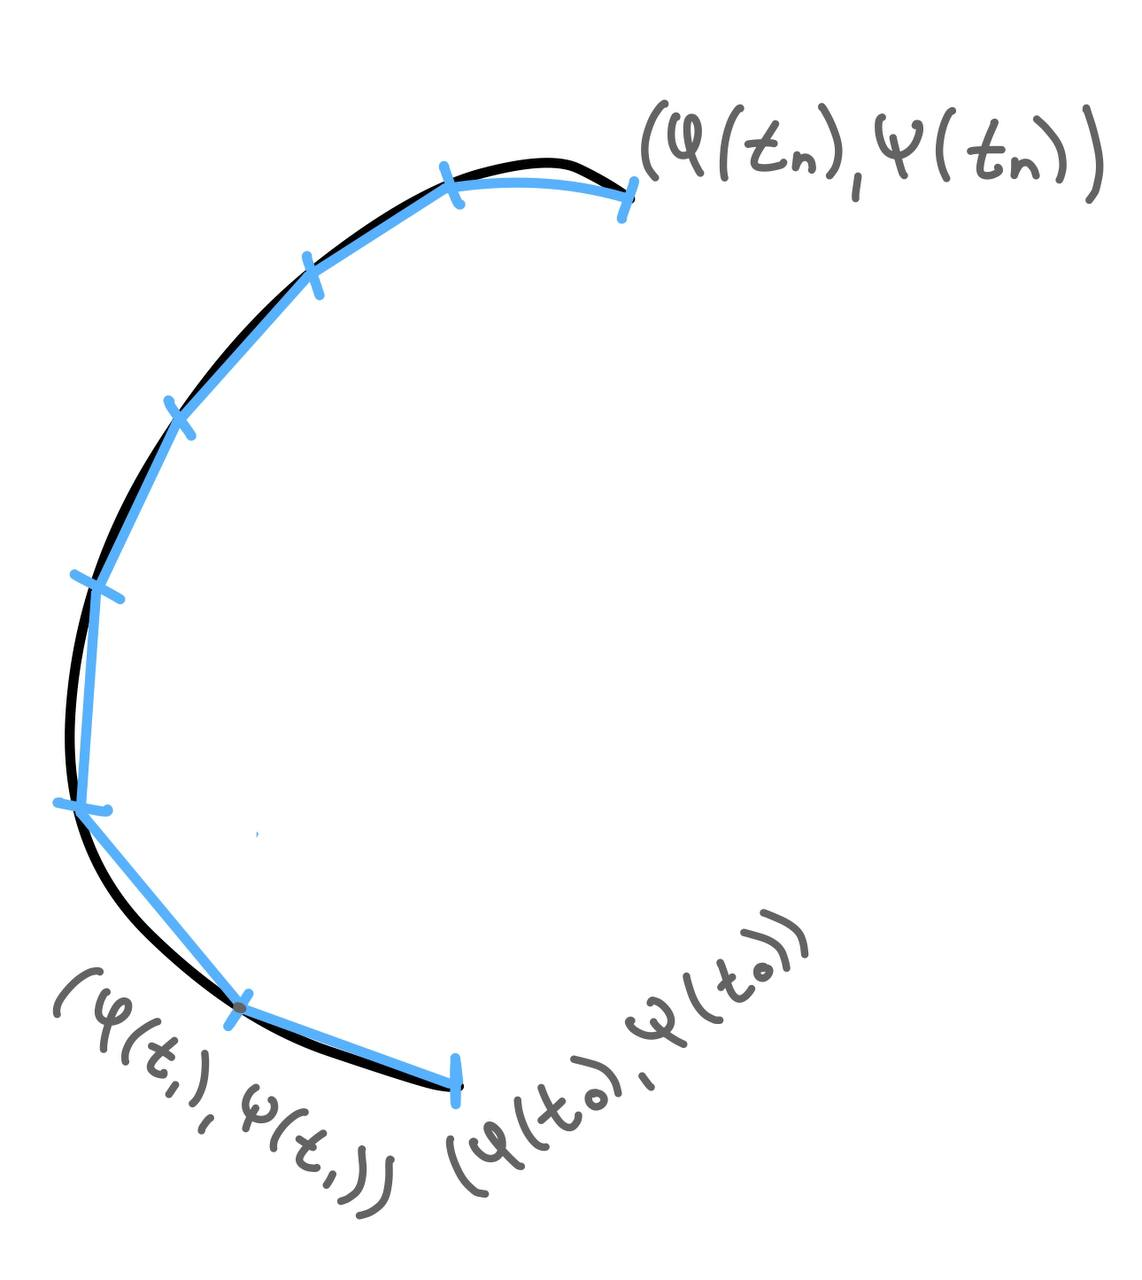
\includegraphics[width=0.4\linewidth]{source/3.png}
    \label{fig:enter-label}
\end{figure}
\newpage
\subsection*{Замечания. (без доказательства)}
1) Всякая гладкая кривая допускает \textbf{параметризацию}.

2) Длина криво обладжает свойствой \textbf{аддитивности}.

Т.е, если \(l_1\) - длина кривой \(\gamma\) между точками \(A\) и \(B\), \(l_2\) - длина кривой между точками \(B\) и \( С\), то \(l = l_1 + l_2\) - длина кривой \(\gamma\) между  точками \(A\) и \(С\)
\begin{figure}[h!]
    \centering
    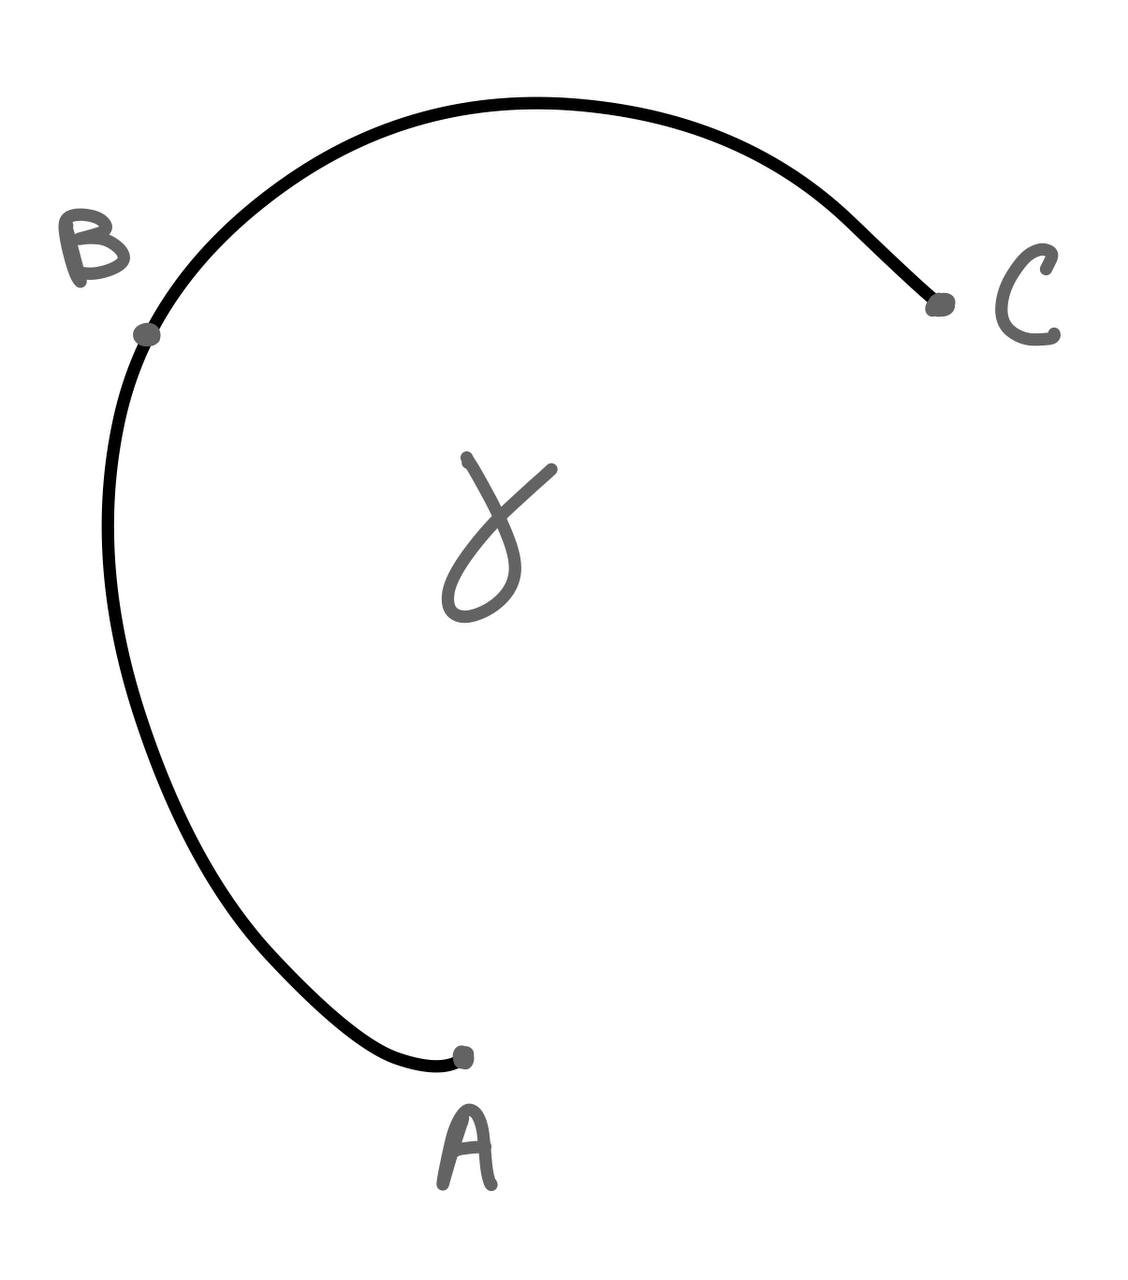
\includegraphics[width=0.4\linewidth]{source/4.png}
    \label{fig:enter-label}
\end{figure}
}